\chapter{Motion planning}

This chapter will focus on the motion planning part. You will learn how to select the motion planner you want (RRT, RRT*, STOMP, CHOMP...), how to create a planning problem and how to solve it.

\section{GUI utilisation}

We can directly use the GUI to solve some motion planning problems. Indeed, moveit has an interface in rviz. Using the GUI will be usefull when you want to quickly test your robot motion or a planning problem. It can also show how long it will last for the motion planner you selected to find a motion plan. However, when you will need to find precise plan (with exact coordinate for joints) or when you will want to generate a lot of trajectories it will be far easier to use scripts.

Using the GUI is really simple. First go to the \emph{motion planning} tab and click on the \emph{planning} tab after (figure \ref{fig:gui_procedure_1}). In this tab you can select your start state and your goal state. Initially the start state should be initialized with the current position of your robot which should be its home position. However, if it not the case you can initialize it yourself by clicking on the \emph{select start state} tab and clicking on the \emph{update} button (the current option should be selected) as shown in figure \ref{fig:gui_procedure_2}. You can see that you can choose other ways to initialize the start goal. For instance you can decide to select a random valid position or pre-determined position. The pre-determined position are generated with the moveit initialization procedure. If you use the motoman project it should have only two pre-determined position : the home position and the up position. As for the goal position, you can either do the same as the start position (selecting random position or pre-determined ones) or just use your mouse and move the robot through the light blue ball inside the gui (see figure \ref{fig:gui_end_effector}). 
\begin{figure}
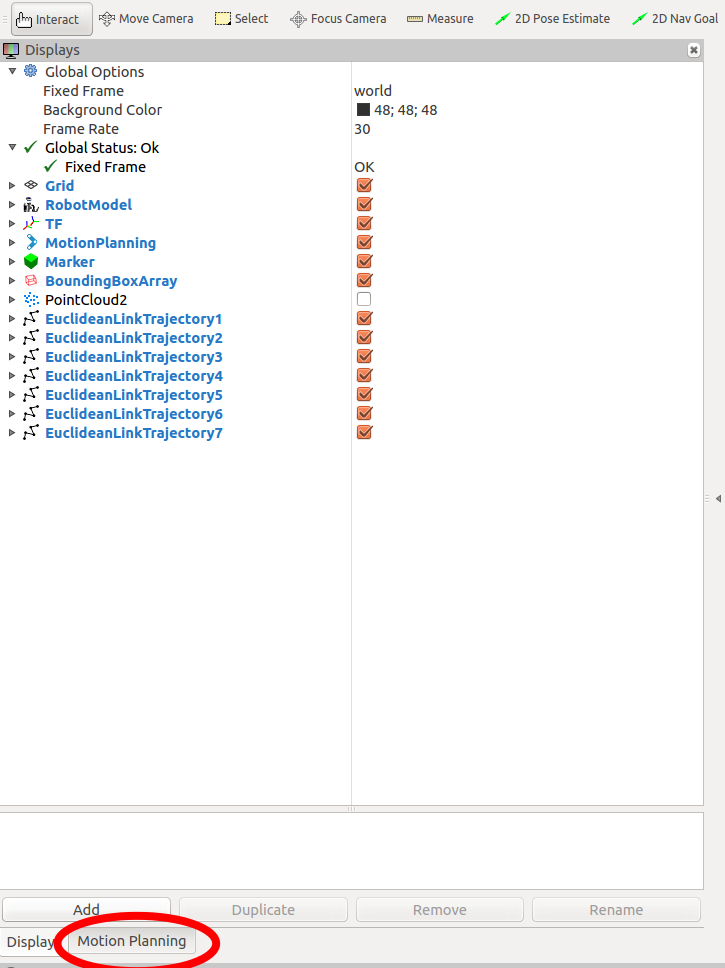
\includegraphics[scale=0.23]{images/motion_planning/gui_moving_procedure_1.png}
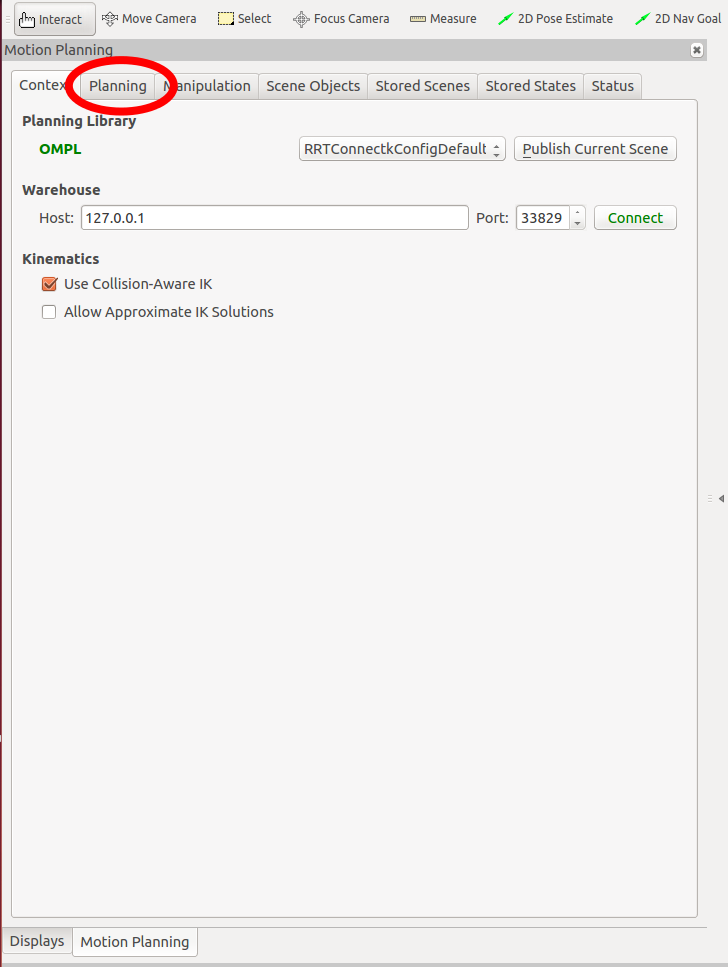
\includegraphics[scale=0.23]{images/motion_planning/gui_moving_procedure_2.png}
\centering
\caption{Clicking on \emph{motion planning}, then \emph{planning}.}
\label{fig:gui_procedure_1}
\end{figure}



\begin{figure}
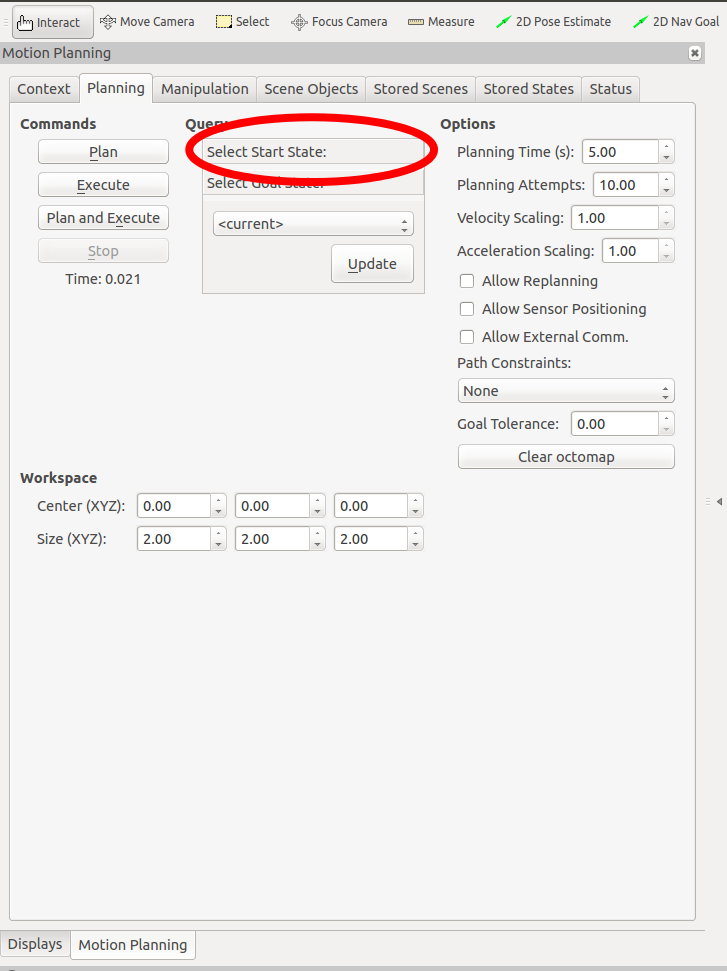
\includegraphics[scale=0.23]{images/motion_planning/gui_moving_procedure_3.png}
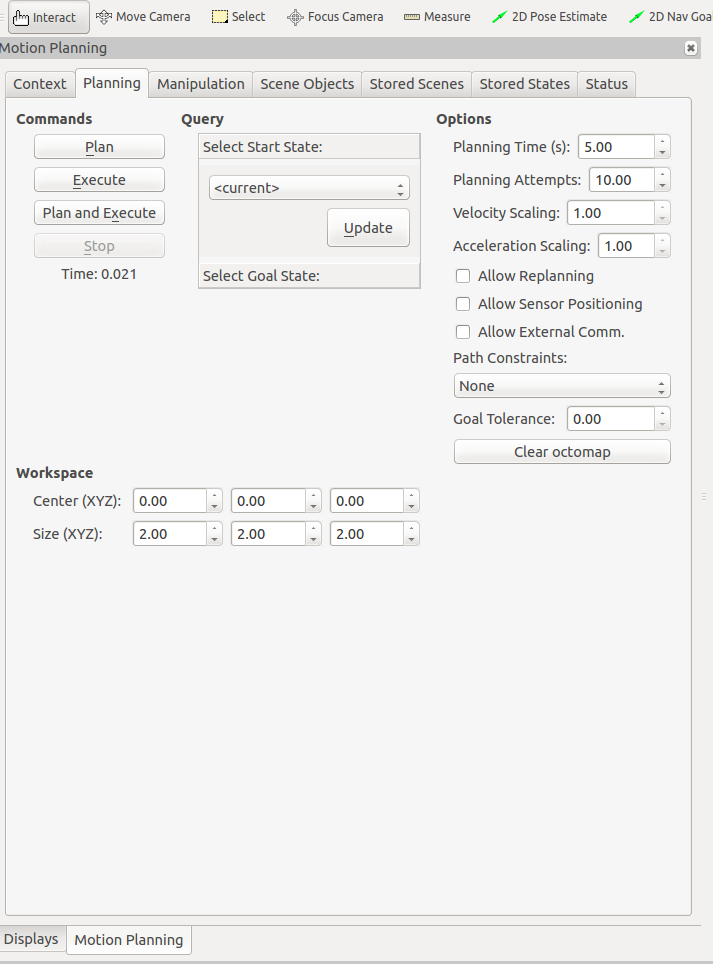
\includegraphics[scale=0.23]{images/motion_planning/gui_moving_procedure_4.png}
\centering
\caption{Clicking on \emph{select start state} and then the \emph{update} button.}
\label{fig:gui_procedure_2}
\end{figure}

\begin{figure}
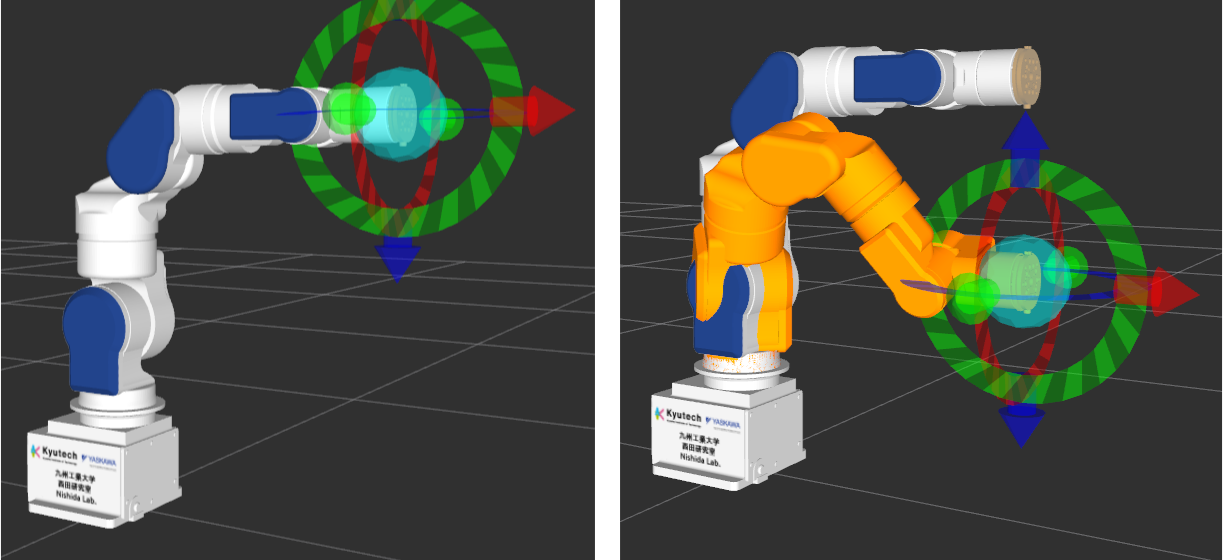
\includegraphics[scale=0.23]{images/motion_planning/gui_end_effector.png}
\centering
\caption{Changing the goal position by moving the end effector ball through the GUI.}
\label{fig:gui_end_effector}
\end{figure}

When you have chosen your start and goal position you just need to click on the \emph{plan} button to try to find a motion plan. If you click on \emph{plan and execute} you will see your robot moving after having successfully found a plan.


\begin{figure}[ht]
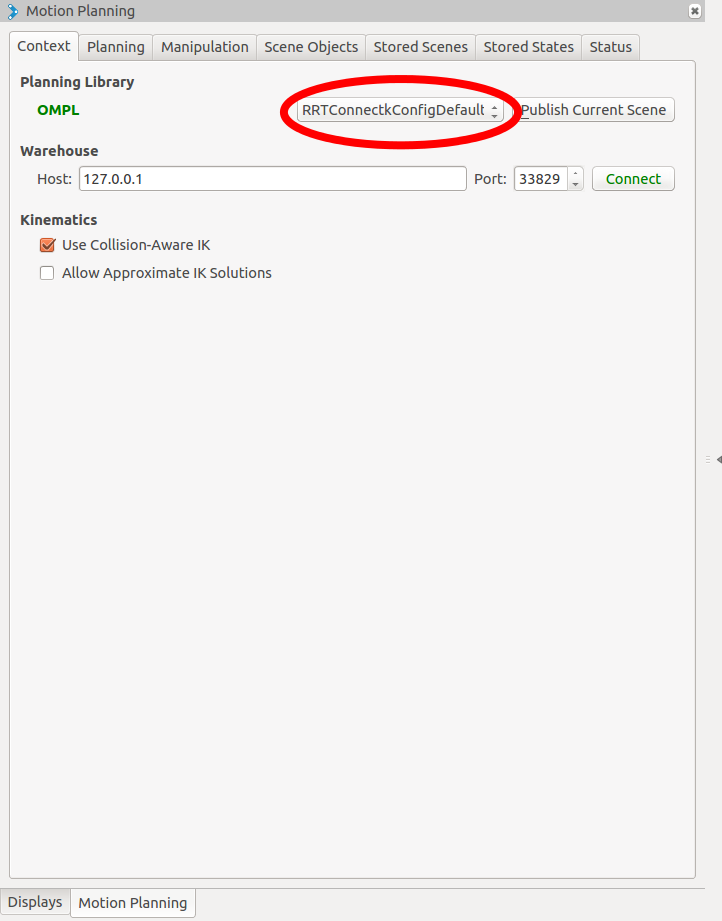
\includegraphics[scale=0.19]{images/motion_planning/gui_change_planner.png}
\centering
\caption{Changing the goal position by moving the end effector ball through the GUI.}
\label{fig:gui_change_planner}
\end{figure}

If you are using the OMPL library you may want to change the motion planner, just click on the tab in the \emph{Planning Library} section (see figure \ref{fig:gui_change_planner}).

\section{Simple script}

In this section we review the script we used during chapter 2 to plan a motion between the home position to a specific position. We will describe the different parts of the code and in the following section we will build on this simple script. The script we used is the following one.

\lstinputlisting[language=c++,caption=moving.cpp]{code_files/motion_planning/moving.cpp}

The first important line is the creation of the object \emph{group}. Moveit will do the interface between the motion planners and the robot but it needs to be initialized to know what robot (or what part of the robot) to work on. In our case the whole parts of the robot will be used and it has been named \emph{arm} during the moveit initialization procedure, that is why we put it as an argument. Then we need to define the start and goal position for our planning problem. In this simple script we define the start position as the current position of the robot. Hence we need to get the current position of the robot with the method \emph{getCurrentState} of our object \emph{group}. For the goal position, we decided to define by ourself the exact position of all the joints of the robot and input it as the goal. To do it we first define a map data structure which will associate for each string (the name of the joint) a double (the joint value). The robot is a 7 degrees of freedom robot so there are 7 joints to give values to. Each joint has a name, you can see in figure \ref{fig:sia5_joints_name} their position with their name. The \emph{setJointValueTarget} method of the object \emph{group} is then the method to call to input the goal position from the previously created map. Eventually we need to call the \emph{plan} method from the \emph{group} object, but this method requires a \emph{Plan} object as argument to store the solution (or nothing if no plan is found). It should be noted that the plan method returns a boolean indicating if a solution has been found or not.

\begin{figure}[ht]
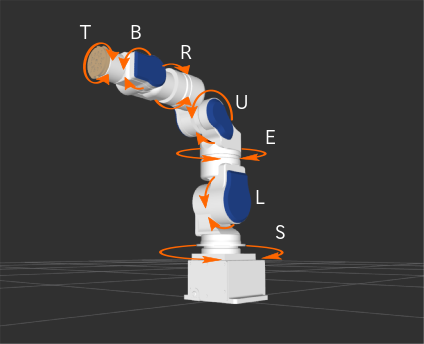
\includegraphics[scale=0.49]{images/motion_planning/robot_model.png}
\centering
\caption{Name of the joints of the robot.}
\label{fig:sia5_joints_name}
\end{figure}

So this script was a really simple one to show the basis of a planning with the moveit library. In the following sections we will show how to add some obstacles in the environment, to change the motion planner and how to do a lot of planning.


\section{Moving to a pose}

Instead of specifying all the joint values it can be useful to just ask the end-effector to be at a defined pose (position and orientation). It is simple to do with moveit but be careful as your specified pose may not be possible to reach by the robot end-effector. The following code is the entire code to plan a motion to a pose goal.

\lstinputlisting[language=c++,caption=moving.cpp]{code_files/motion_planning/moving_to_pose.cpp}

You can see that the only part that changed was the goal state definition compared to the simple script. We first create a \emph{Pose} object and then set its attributes. Finally we inform moveit by using the \emph{setPoseTarget} method. 

However be careful ! If you want to use the STOMP planner you cannot only specify a pose, you will need to transform it to joint space. You can do it by adding the following code.

\begin{lstlisting}[language=c++]
robot_state::RobotState robot_state_goal(*group.getCurrentState());
std::map<std::string, double> joints;
joints["joint_s"] = robot_state_goal.getVariablePosition("joint_s");
joints["joint_l"] = robot_state_goal.getVariablePosition("joint_l");
joints["joint_e"] = robot_state_goal.getVariablePosition("joint_e");
joints["joint_u"] = robot_state_goal.getVariablePosition("joint_u");
joints["joint_r"] = robot_state_goal.getVariablePosition("joint_r");
joints["joint_b"] = robot_state_goal.getVariablePosition("joint_b");
joints["joint_t"] = robot_state_goal.getVariablePosition("joint_t");
group.setJointValueTarget(joints);
\end{lstlisting}

\section{Changing the start state}
Sometimes it can be useful to change the start state instead of the goal state (or you can change both !). In this case there are two ways to do it. You can either specify a pose and use inverse kinematics to find the joint values like in the following code.
 

\begin{lstlisting}[language=c++]
robot_state::RobotState robot_state_start(*group.getCurrentState());
geometry_msgs::Pose start_pose;
  
start_pose.orientation.w = 1.0; 
start_pose.orientation.w = 1.0;
start_pose.position.x = 0.45;
start_pose.position.y = 0.1;
start_pose.position.z = 0.65;
  
const robot_state::JointModelGroup *joint_model_group =
  robot_state_start.getJointModelGroup(group.getName());
  
robot_state_start.setFromIK(joint_model_group, start_pose);
group.setStartState(robot_state_start);
\end{lstlisting}

Or you can directly change the joint values by using the next code.


\begin{lstlisting}[language=c++]
robot_state::RobotState robot_state_start(*group.getCurrentState());
    
std::vector<double> start_joints(7);

for(int i=0;i<7;i++) {
	start_joints[i]=0.2;
}
      
robot_state_start.setVariablePositions(start_joints);
group.setStartState(robot_state_start);
\end{lstlisting}




\section{Moving to a random pose}

Sometimes it could be useful to ask the robot to go to a random pose. In moveit it is easy to do it and the answer will be a reachable pose (not a pose with collisions or out of the reach of the robot). You just need to add the following line.

\begin{lstlisting}[language=c++]
group.setRandomTarget();
\end{lstlisting}

However, even if asking for a random target is easy it is rather difficult to do a random start (will explain in future version of this manual).

\section{Changing motion planner}

If you want to use an other motion planner than the default one you can do it quite easily ! If the motion planner you want to use is inside OMPL then you simply need to use the method \emph{setPlannerId} with the name of the planner for attribute. For instance, if you want to use the TRRT motion planner just add the following line.


\begin{lstlisting}[language=c++]
group.setPlannerId("TRRTkConfigDefault");
\end{lstlisting}

Here is the list of planner's name you can use :
\begin{itemize}
\item SBLkConfigDefault
\item ESTkConfigDefault
\item LBKPIECEkConfigDefault
\item BKPIECEkConfigDefault
\item KPIECEkConfigDefault
\item RRTkConfigDefault
\item RRTConnectkConfigDefault
\item RRTstarkConfigDefault
\item TRRTkConfigDefault
\item PRMkConfigDefault
\item PRMstarkConfigDefault
\end{itemize}

If you want to use the STOMP planner you cannot use the method \emph{setPlannerId}, instead you will need to modify the launch file. You will need to put \emph{stomp} inside the \emph{planning\_config} argument, \emph{false} for the \emph{use\_ompl} argument and \emph{true} for the \emph{use\_stomp} argument like the following. 



\begin{lstlisting}
<!-- Choose planner [ompl|chomp|stomp] -->
<arg name="planning_config" default="stomp"/>
<!-- If you choose ompl, "use_ompl" is true. -->
<arg name="use_ompl" default="false"/>
<!-- If you choose stomp, "use_stomp" is true. -->
<arg name="use_stomp" default="true"/>
\end{lstlisting}


\section{Adding an obstacle}
\subsection{A simple box}

The previous scripts we have shown are a bit boring without any obstacle. In this section we will explain how to add an obstacle which will be visible in Rviz. First you will need to include the \emph{planning\_scene\_interface.h} file and create a \emph{PlanningSceneInterface} object. This object will be used to add obstacle in the moveit environment. Then you will need to create a vector which will contain all the obstacles you want to add. An obstacle is a \emph{CollisionObject} object, it will need a unique to be identified. In this simple example we choose to add a box as obstacle, you should then first define its dimensions. When the shape of the obstacle has been defined (in this case a box) you will need to define its pose in the environment. In this example we only choose its $(x,y,z)$ coordinates but you can also choose its orientation. Once it has been done you can simply use the \emph{push\_back} method of the obstacle to add its primitive and pose information. Finally you should add the obstacle to the vector previously created and update the \emph{planning\_scene.
}
The following code illustrate all of this. Note that the goal position has been changed to show that the robot needs to avoid the newly add obstacle.


\lstinputlisting[language=c++,caption=moving.cpp]{code_files/motion_planning/add_obstacle.cpp}


\subsection{Other primitives}
Sometimes you will not want to have obstacle with the shape of a box, you can for example have a bottle near your robot that would be better described as a cylinder rather than a box. Moveit gives you in four basic shapes : box, sphere, cylinder and cone. However you can also add a more complicated primitive by using meshes. When you want to use another primitive than the box you will only need to change the primitive part of the code, there is no need to change the position and orientation part.

If you want to use a sphere you will need first to resize the dimension of your primitive to $1$. Indeed, a sphere is entirely described by its radius, so there is only $1$ parameter required. The following code shows how to change the box to a sphere with a $0.04m$ radius .

\begin{lstlisting}[language=c++]
shape_msgs::SolidPrimitive primitive;
primitive.type = primitive.SPHERE;
primitive.dimensions.resize(1);
primitive.dimensions[0] = 0.04; // radius
\end{lstlisting}

If you prefer a cylinder, it is almost the same except that you will need two parameters : one for the height and one for the radius.


\begin{lstlisting}[language=c++]
shape_msgs::SolidPrimitive primitive;
primitive.type = primitive.CYLINDER;
primitive.dimensions.resize(2);
primitive.dimensions[0] = 0.04; // height
primitive.dimensions[1] = 0.2;  // radius
\end{lstlisting}

Finally,  if you want a cone you will also need two parameters : one for the height and one for the radius of the base.

\begin{lstlisting}[language=c++]
shape_msgs::SolidPrimitive primitive;
primitive.type = primitive.CONE;
primitive.dimensions.resize(2);
primitive.dimensions[0] = 0.04; // height
primitive.dimensions[1] = 0.2;  // radius
\end{lstlisting}